%\documentclass[handout]{beamer}
\documentclass{beamer}
\usepackage{array}
\usepackage{graphicx}
\usepackage{german}
%\usepackage{txfonts}

\mode<beamer>{%
\usetheme[hideothersubsections,hidetitle]{Hannover}
}
\title[]{Partielle Differentialgleichungen}
\subtitle{4. Sitzung: Separation II, Transformation}
\date[11.~M"arz 2015]{11.~M"arz 2015}
\author{Prof.~Dr.~Andreas M"uller}
\begin{document}

\begin{frame}
\section{Separation}
\titlepage
\end{frame}

\begin{frame}
\frametitle{Zusammenfassung: Separation}
\begin{enumerate}[<+->]
\item Koordinaten: m"ussen zu Gebietsgrenzen passen
\item Separationsansatz: 
\begin{align*}
&\text{meistens:}&u(x,y)&=X(x)\cdot Y(y)\\
&\text{manchmal:}&u(x,y)&=X(x)+Y(y)
\end{align*}
\item Einsetzen und Variablen trennen
\[
\text{nur $x$} = \text{nur y}\quad\Rightarrow\quad \text{beide konstant $=\mu$}
\]
$\Rightarrow$ Eigenwertproblem
\item Nullrandbedingungen legen $\mu$ fest: $\mu_1$, $\mu_2$,
$\mu_3,\dots,\mu_n,\dots$
\item Teill"osungen $u_n(x,y)=X_n(x)\cdot Y_n(y)$  zu jedem $\mu_n$
\item "Uberlagerung (nur f"ur lineare PDGL)
\[
u(x,y)=\sum_n a_nu_n(x,y)
\]
\item Koeffizienten $a_n$ aus verbleibenden Randbedingungen
\end{enumerate}
\end{frame}

\begin{frame}
\section{Tsunami}
\frametitle{Sendai-Erdbeben}
\begin{center}
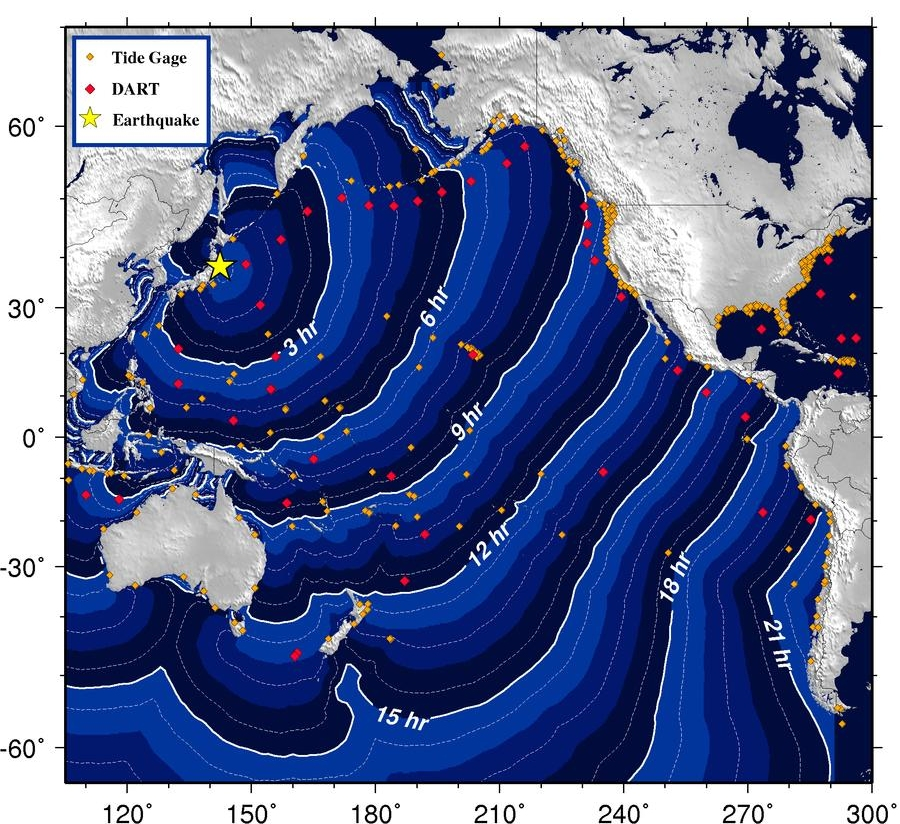
\includegraphics[width=0.85\hsize]{../../skript/graphics/sendainoaa.jpg}
\end{center}
\end{frame}

\begin{frame}
\frametitle{Tsunami}
{\bf Wellengleichung} auf der Kugeloberfl"ache:
\[
\frac{1}{c^2}\frac{\partial^2u}{\partial t^2}
=
\Delta u
\]
\pause
{\bf Kugel-Koordinaten:} $(r,\vartheta,\varphi)$,
d.~h.~$u(t,r,\vartheta,\varphi)$

\medskip
\pause
{\bf Laplaceoperator:}
\[
\Delta = \frac{1}{r^2}\frac{\partial}{\partial r}r^2\frac{\partial}{\partial r}
+
\frac{1}{r^2\sin\vartheta}\frac{\partial}{\partial\vartheta}\sin\vartheta\frac{\partial}{\partial\vartheta}
+
\frac1{r^2\sin^2\vartheta}\frac{\partial^2}{\partial\varphi^2}
\]
{\bf Symmetrie:}
\begin{enumerate}
\item Unabh"angig von $r$, d.~h.~$r=1$
\item Rotationssymmetrie um Epizentrum
\end{enumerate}
\pause
{\bf Randbedingungen:}
\begin{align*}
\frac{\partial u}{\partial\vartheta}(t,0)&=0
&
u(0,\vartheta)&=F(\vartheta)
\\
\frac{\partial u}{\partial\vartheta}(t,\pi)&=0
&
\frac{\partial u}{\partial t}(0,\vartheta)&=G(\vartheta)
\end{align*}

\end{frame}

\begin{frame}
\frametitle{L"osung}
\begin{enumerate}[<+->]
\item Ansatz: $u(t,\vartheta)=T(t)\cdot \Theta(\vartheta)$
\item Separation:
\[
\frac{1}{c^2}\frac{T''(t)}{T(t)}
=
m
=
\frac{1}{\Theta(\vartheta)\sin\vartheta}\frac{\partial}{\partial\vartheta}\sin\vartheta
\Theta'(\vartheta)
\]
\item L"osung f"ur $T(t)$:
\[
T_m(t)=\cos\sqrt{-m}t
\qquad\text{oder}\qquad
T_m(t)=\sin\sqrt{-m}t
\]
\item L"osung f"ur $\Theta(\vartheta)$: Polynom $P_k(\cos\vartheta)$,
$m_k=-k(k+1)$
\item Allgemeine L"osung: "Uberlagerung
\[
u(t,\vartheta)=
\sum_{k=0}^\infty
(a_k\cos\sqrt{-m_k}t+b_k\sin\sqrt{-m_k}t)P_k(\cos\vartheta)
\]
\item Anfangsbedingungen: Fouriertheorie f"ur Legendre-Polynome
\end{enumerate}

\end{frame}

\begin{frame}
\frametitle{L"osung $\Theta(\vartheta)$}
\begin{enumerate}
\item Substition $z=\cos\vartheta$, $y(z)=\Theta(\cos\vartheta)$
\item Legendre-Differentialgleichung:
\[
\frac{d}{dz}(1-z^2)\frac{d}{dz}y(z) =my(z).
\]
\item Fall $m=0$:
\[
y(z)=\frac{C}2\frac{1+z}{1-z}+D
\]
\item Allgemeiner Fall: Legendre-Polynome $P_k^l(z)$, aber nur
f"ur $m_k=-k(k+1)$, $k\in\mathbb N$ und $l=0,1,\dots,n$.
Wir brauchen nur $l=0$.
\end{enumerate}
\end{frame}

\begin{frame}
\frametitle{Approximation}
\begin{center}
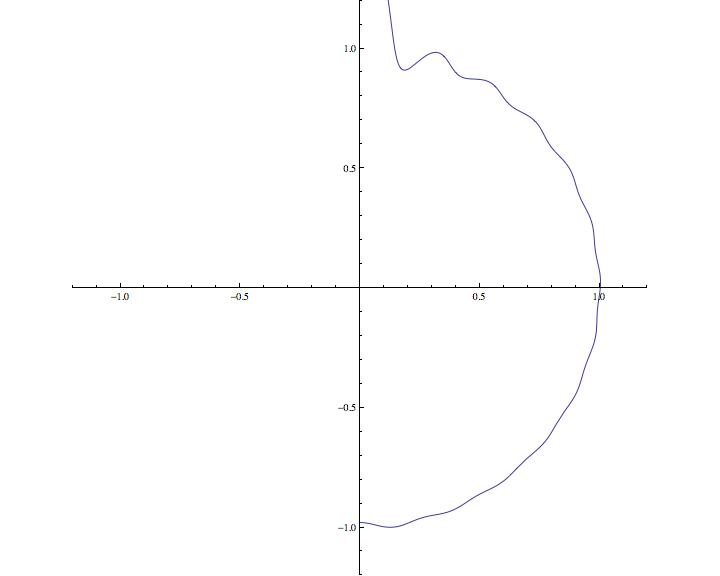
\includegraphics[width=0.9\hsize]{../../skript/graphics/tsunami0.jpg}
\end{center}
\end{frame}

\begin{frame}
\frametitle{Approximation}
\begin{center}
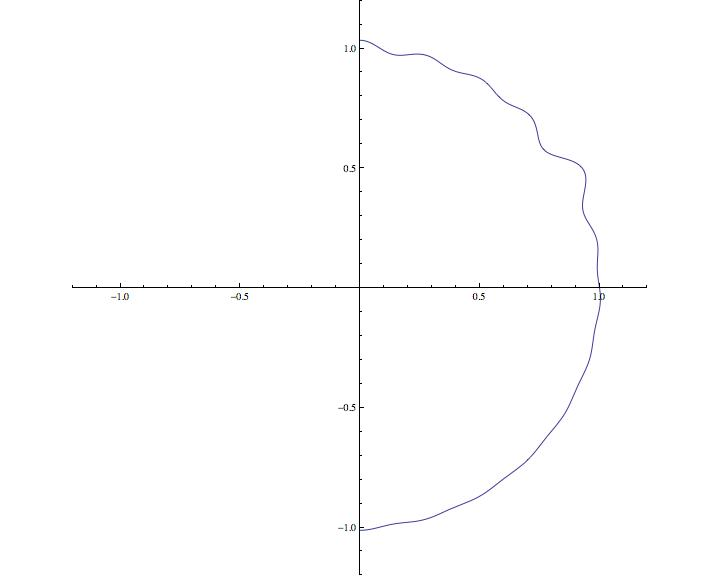
\includegraphics[width=0.9\hsize]{../../skript/graphics/tsunami50.jpg}
\end{center}
\end{frame}

\begin{frame}
\section{Transformation}
\frametitle{Transformation}

{\bf Beobachtung:} Separation f"uhrt auf $\sin kx$ und $\cos kx$,
d.~h.~Fourier-Reihen.

\[
\Rightarrow
\]
\bigskip

{\bf Idee:} Fourier-Reihen von Anfang an verwenden!

\end{frame}

\begin{frame}
\frametitle{Fourier-Transformation}

Jede Funktion $f\colon [0,2\pi]\to\mathbb R$ kann als Fourier-Reihe
geschrieben werden:
\[
f(x)=\frac{a_0}{2}+\sum_{k=1}^\infty(a_k\cos kx+b_k\sin kx).
\]

\medskip
\pause
Dies definiert die Fouriertransformation
\medskip

\begin{align*}
{\cal F}\colon
f
&\mapsto
a_0, a_k, b_k, k> 0
\end{align*}

\end{frame}

\begin{frame}
\frametitle{Ableitungen}
$a_0$, $a_k$, $b_k$ Fourier-Koeffizienten von $f$.

\[\Rightarrow\]

Fourierkoeffizienten der Ableitung nach $x$
\begin{align*}
f'(x)&=\sum_{k=1}^\infty (-ka_k\sin kx+kb_k\cos kx)\\
f''(x)&=\sum_{k=1}^\infty (-k^2a_k\cos kx-k^2b_k\sin kx)
\end{align*}
Ableitungsoperator f"ur Fourierkoeffizienten:
\begin{align*}
a_k&\mapsto -k^2a_k\\
b_k&\mapsto -k^2b_k\\
\end{align*}
\end{frame}

\begin{frame}
\frametitle{Funktion von $x$ und $t$}

$u$ eine Funktion von $x$ und $t$:
\[
u\colon (0,2\pi)\times \mathbb R^+\to \mathbb R
\]
Fourierkoeffizienten h"angen von $t$ ab:
\[
u(x,t)=\frac{a_0(t)}2+\sum_{k=1}^\infty (a_k(t)\cos kx+b_k(t)\sin kx)
\]
Fourier-Transformation
\[
{\cal F}\colon
u\mapsto
a_0(t), a_k(t), b_k(t)
\]
\pause
Implizite Separation:
\begin{enumerate}[<+->]
\item Ortsabh"angigkeit in $\cos kx$ und $\sin kx$
\item Zeitabh"angigkeit in $a_k(t)$ und $b_k(t)$
\end{enumerate}

\end{frame}

\begin{frame}
\frametitle{Differentialgleichung}

Wellengleichung:
\[
\frac{1}{c^2}
\frac{\partial^2 u}{\partial t^2}
=
\frac{\partial^2 u}{\partial x^2},
\]
Gebiet:
\[
\Omega = (0,2\pi)\times \mathbb R^+\to \mathbb R
\]
Randbedingungen:
\begin{align*}
u(t,    0)&= 0&u(0,x)&=f(x)\\
u(t, 2\pi)&= 0&\frac{\partial}{\partial t}u(0,x)&=g(x)
\end{align*}
Fourierkoeffizienten von $f$ und $g$: $b_k^{(f)}$ und $b^{(g)}_k$

\end{frame}

\begin{frame}
\frametitle{Transformation}
Randbedingungen:
\[
a_0=0\qquad
a_k=0\;\forall k > 0
\]
Differentialgleichung:
\begin{align*}
\frac{1}{c^2}\ddot b_k(t)&= -k^2b_k(t)
\end{align*}
Anfangsbedingung:
\begin{align*}
b_k(0)&= b_k^{(f)}& \dot b_k(0)&=b_k^{(g)}
\end{align*}
{\bf Gew"ohnliche} Differentialgleichungen f"ur die Fourier-Koeffizienten
\end{frame}

\end{document}
